\chapter{Courbes elliptiques}
    \section{Motivation}
        Algos qui reposent sur le problème du log discret :
        \begin{itemize}
            \item El Gamal 1987 (chiffrement et signature)
            \item DSA (Digital Signature Algorithm) standardisé par le NIST (variante d'El Gamal)
            \item Diffie-Hellman
        \end{itemize}
        V. Miller, N. Koblitz (1982) ont l'idée d'utiliser les courbes elliptiques en crypto.

        \subsection{Diffie-Hellman}
            $p$ premier, $g$ générateur de $\mathbb{F}_p^*$.
            \begin{figure}[H]
                \centering
                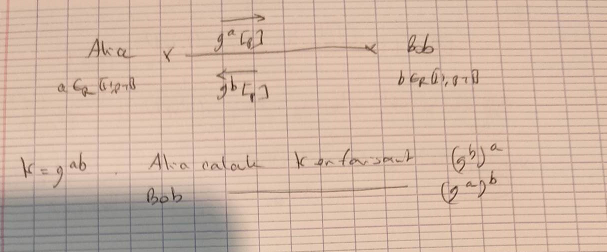
\includegraphics[width=.5\textwidth]{pictures/13}
            \end{figure} \noindent 
            Sécurité de Diffie-Hellman
            \begin{itemize}
                \item Attaques passives : a partir de $p, g, g^a [p], g^b [p]$, trouver $g^{ab} [p]$ (problème Diffie-Hellman). Si on sait retrouver $a$ à partir de $g, p, g^a [p]$ (problème du log discret), alors on sait résoudre le problème D-H. On ne sait pas cependant si ces deux problèmes sont équivalents.*
                \item Attaque man in the middle :
                \begin{figure}[H]
                    \centering
                    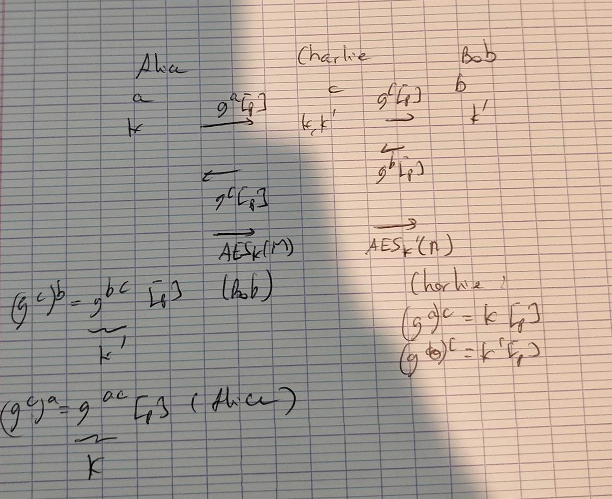
\includegraphics[width=.5\textwidth]{pictures/14}
                \end{figure} \noindent
                Pour résoudre le problème, on fait un DH authentifié
                \begin{figure}[H]
                    \centering
                    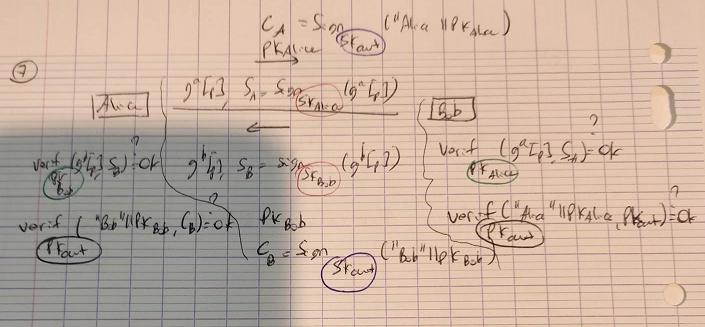
\includegraphics[width=.5\textwidth]{pictures/15}
                \end{figure} \noindent
            \end{itemize}

        \subsection{Groupe}
            Diffie-Hellman "historique", on utilise $\znz{p}^*$. Pour généraliser, on a besoin d'un groupe $G$, d'un générateur $g$ de $G$, dans lequel le problème du log discret est difficile. Remarquons qu'il faut aussi que les éléments de $G$ aient une représentation qui permette de faire facilement des calcules DH. Le protocole est réalisé comme pour le cas $\mathbb{F}_p^*$. Il y a des groupes qui sont complètement inutilisables, du faut que le problème du log discret est facile dedans : par exemple, $\znz{p}$ muni de l'addition ne convient pas puisque le problème du log discret se traduit comme trouver $a$ lorsque l'on connait $ag [p]$. Le cas historique utilise $G = \mathbb{F}_p^*$, mais remarquons qu'il peut être difficile de trouver un générateur d'un tel groupe.
            
        \subsection{Quels sont les groupes dans lesquels le log discret est difficile ?}
            \begin{remq}
                Baby step giant step : $y = g^a$, écrivons $a = tq + r$ avec $t = \sqrt{\card{G}}
                $. Alors $yg^{-tq} = g^r$, et avec le paradoxe des anniversaires/baby step giant step on obtiens un algo en $\mathcal{O}(\sqrt{\card{G}})$ (et comme cet algo est généraliste on ne peut pas espérer une complexité supérieure pour le problème du log discret dans un groupe $G$).
            \end{remq}

    \section{Courbes elliptiques}
        \subsection{Définition}
            Courbes sur $\mathbb{R}$ : équation de Weierstrass $y^2 = x^3 + ax + b$. 

        \subsection{Formules d'addition}
            On calcule $R = P + Q$ de la manière suivante :
            \begin{align*}
                &u =
                \begin{cases}
                    &\frac{y_Q - y_P}{x_Q - x_P} \\
                    &\frac{3x_P^2 + a}{2y_P} \\
                \end{cases} \\
                &v = y_P - ux_P \\
                &x_R = u^2 - x_P - x_Q \\
                &y_R = -(ux_R + v)
            \end{align*}

        \subsection{Coordonnées projectives}

        \subsection{Nombre de points sur $E$}
            $E : \{(x,y) \in (\mathbb{F}_p)^2 \mid y^2 = x^3 + ax + b\} \cup \{\mathcal{O}\}$. C'est un groupe commutatif.
            \begin{prop}
                Si $p > 2$, le nombre d'éléments de $\mathbb{F}_p^*$ qui sont des carrés est $\frac {p-1}2$.
            \end{prop}
            \begin{proof}
                Considérons
                \begin{align*}
                    \begin{array}{cccc}
                        g : & \mathbb{F}_p^* & \to & \mathbb{F}_p^* \\
                        & u & \mapsto & u^2 \\
                    \end{array}
                \end{align*}
                est un morphisme de groupe, de noyau $\{-1, 1\}$. Ainsi $\card{\im g} = \card{\mathbb{F}_p^*} / \card{\ker g} = \frac{p - 1}2$
            \end{proof}
            \begin{prop}
                $p > 2$, $x \in \mathbb{F}_p^*$ est un carré si et seulement si $x^{\frac{p - 1}2} = 1$.
            \end{prop}
            \begin{proof}
                Clairement, si $x$ est un carré, alors $x^{\frac{p - 1}2} = 1$. Et $X^{\frac{p - 1}2} - 1$ a comme racines tous les carrés de $\mathbb{F}_p^*$, qui sont au nombre de $\frac{p - 1}2$, et vu son degré ce sont exactement les racines, ce qui prouve l'implication réciproque.
            \end{proof}
            \begin{prop}
                Si $p = 3 [4]$ et si $x \in \mathbb{F}_p^*$ est un carré, alors $x = u^2$ avec $u = x^{\frac{p + 1}4}$.
            \end{prop}
            \begin{proof}
                \begin{align*}
                    u^2 = \left( x^{\frac{p + 1}4} \right)^2 = x^{\frac{p + 1}2} = x^{\frac{p - 1}2} x = x
                \end{align*}
            \end{proof}
            \begin{remq}
                En général, si $p$ est premier quelconque, alors on dispose de l'algorithme de Shanks pour trouver une racine carrée.
            \end{remq}

            \subsubsection{Heuristique}
                $E : y^2 = x^3 + ax + b$,
                \begin{align*}
                    \card{E} &= \card{\{x \in \mathbb{F}_p \mid x^3 + ax + b \text{ est un carré dans } \mathbb{F}_p^*\}} \times 2 + \card{\{x \in \mathbb{F}_p \mid x^3 + ax + b = 0\}} + 1 \\
                \end{align*}
                Au vu de ce calcul, on peut estimer que $|E| \simeq p + 1$
                \begin{theo} (Hasse, 1940)
                    \begin{align*}
                        p + 1 - 2\sqrt{p} \leq \card{E} \leq p + 1 + 2 \sqrt{p}
                    \end{align*}
                \end{theo}
                \begin{theo} (Deuring)
                    Tous les points entiers de $[p + 1 - 2\sqrt{p}, p + 1 + 2\sqrt{p}]$ sont effectivement le cardinal d'une certaine courbe.
                \end{theo}
                On peut même essayer d'étudier les valeurs de $|E|$, c'est la conjecture de Sato-Tate (démontrée par R.Taylor). On dispose aussi d'algorithmes efficaces pour calculer le nombre d'éléments sur une courbe elliptique : SEA, AGM.

    \section{Diffie-Hellman sur courbes elliptiques (ECDH)}
        \subsection{Description}
            $G = (E, +)$ courbe ellipitiques sur $\mathbb{F}_p$. On suppose de plus qu'on dispose de $P \in E$ qui est un générateur.
            \begin{figure}[H]
                \centering
                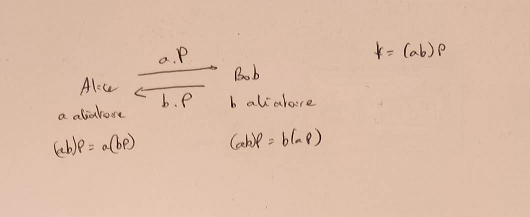
\includegraphics[width=.5\textwidth]{pictures/2_1}
            \end{figure} \noindent
            \begin{figure}[H]
                \centering
                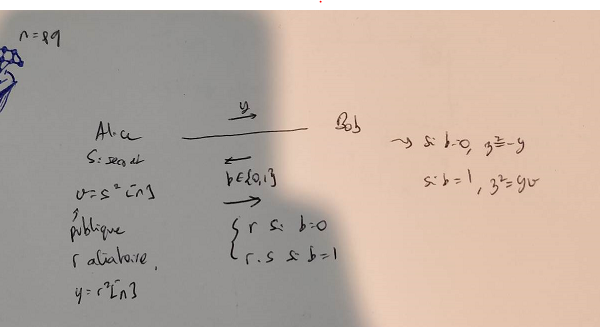
\includegraphics[width=.5\textwidth]{pictures/2_2}
            \end{figure} \noindent

        \subsection{Implémentation}
            "double and add" : on veut calculer $aP$, on écrit $a = \sum a_i2^i$.
            \begin{algorithm}
                \caption{Calcule $aP$ sur une courbe elliptique}
                \begin{algorithmic}
                    \Function{Double and add}{$a, P$}
                        \State $Q \gets 0$
                        \For{$i$ de $k - 1$ à $0$}
                            \State $Q \gets 2Q$
                            \If{$a_i = 1$}
                                \State $Q \gets Q + P$
                            \EndIf
                        \EndFor
                        \State \Return $Q$
                    \EndFunction
                \end{algorithmic}
            \end{algorithm}
            
        \subsection{Sécurité ECDG}
            Repose sur la difficulté du log discret sur $E$, cad trouver $a$ a partir de $P$ et $aP$. Le meilleur algorithme connu est en $\mathcal{O}(\sqrt{\card{E}}) = \mathcal{O}(\sqrt{P})$. Ainsi il faut $\sqrt{p} \geq 2^{128}$, donc $p$ de taille $256$ bits.
            \begin{remq}
                Les couplages (pairings)
                \begin{itemize}
                    \item A. Joux (2001) : DH tripartite
                    \item Boneh, Franklin : chiffrement basé sur l'identité 
                \end{itemize}
            \end{remq}

        \subsection{Comparaison}
            \begin{figure}[H]
                \centering
                \begin{tabular}{c|c|c}
                    & DH & ECDH \\
                    \hline
                    Alice & $g^a [p]$, $(g^b)^a[p]$ & $aP$, $a(bP)$ \\
                    \hline
                    Bob & $g^b [p]$, $(g^a)^b[p]$ & $bP$, $b(aP)$ \\
                    \hline
                    $p$ & 3000 bits & 256 bits \\
                    \hline
                    $K$ & 3000 bits & 256 bits \\
                    \hline
                    Communication & 3000 bits de alice vers bob & $256 + 1$ bits (l'abscisse et quelle \\
                    && racine carrée prendre pour $y$) \\
                \end{tabular}
            \end{figure} \noindent

    \section{Signature}
        \subsection{El Gamal}
            $p$ nombre premier, $g$ générateur de $\Fps$. $x$ secret, $y = g^x [p]$ est publique. On dispose d'une fonction de hachage $h : \{0, 1\}^* \to \znz{(p - 1)}$.
            \begin{description}
                \item[Signature d'un message $M$ :] 
                    \begin{itemize}
                        \item $k$ aléatoire
                        \item $r = g^k [p]$
                        \item $s = k^{-1}(h(M) - xr) [p - 1]$
                    \end{itemize}
                \item[Vérification :] On vérifie que $y^rr^s = g^{h(M)} [p]$.
            \end{description}

            \subsubsection{Elliptic Curve Digital Signature Algorithm (ECDSA)}
                $E$ courbe elliptique, $P$ générateur, $x$ secret et $Q = xP$ est la clé publique. On suppose que l'on dispose d'une fonction de hachage $h : \{0, 1\}^* \to \znz{(p - 1)}$.
                \begin{description}
                    \item[Signature de $M$ :] 
                    \begin{itemize}
                        \item $k$ aléatoire
                        \item $R= kP$
                        \item $r$ est l'abscisse de $R$
                        \item $s = k^{-1} (h(M) + xr) [p - 1]$
                    \end{itemize}
                    \item[Vérification :] Abscisse$\left( \frac{H(M)}s P + \frac rs Q \right) = r$.
                \end{description}